Our project began by creating a small webapp which coordinated the instruction generating process.
This program, also dubbed ``Canned Mentorship,'' consisted of two separate programs:
\begin{enumerate}
	\item a website interface for coordinating working users
	\item a back-end AI script for classifying answers and removing redundant inputs
\end{enumerate}



%webapp description
%theory
%workflow
%implementation

%ai backend
%interface with program
%parameters
	%reasons for choosing
%flow
%
\begin{comment}
\begin{figure}[h]
	\begin{center}
		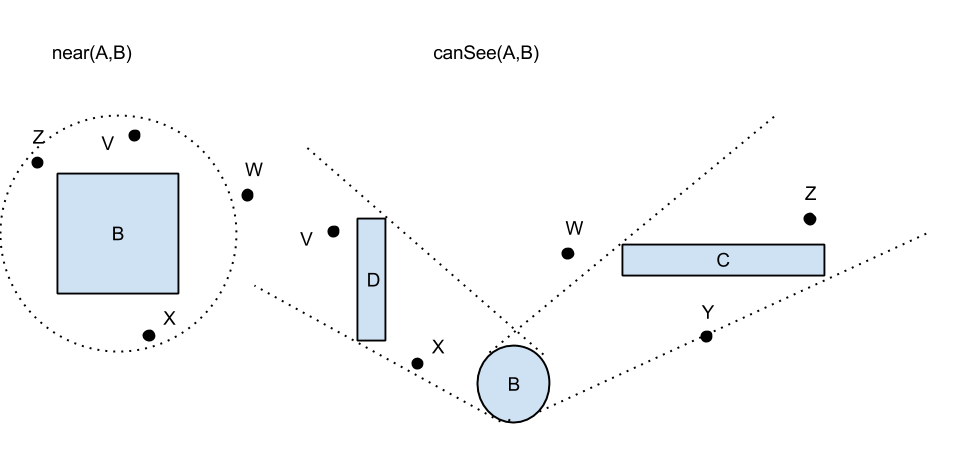
\includegraphics[width=0.48\textwidth]{figures/rejection_sampling_placement.png}
	\caption{Rejection sampling was also considered as a placement mechanism.}
	\label{fig:rejection_sampling_placement}
	\end{center}
\end{figure}
\end{comment}